\chapter{Object Selection}
\label{cha:objsel}

Choosing recipes for selecting well reconstructed physics objects is necessary before one is able to apply analysis requirements. Their general task is to reduce the number of false reconstructions. For example a hadronic fragment can ``punch through'' the HCAL and leave a track in the muon system. This might then be falsely identified as a muon and interfere with the signal. These recipes for object identification (\textbf{ID}) have been developed by the respective physics object groups (\textbf{POG}). In this chapter, the various steps in the decision of deeming an object valid or invalid will be given.

Additional distributions displaying the effects of the individual ID criteria are placed in appendix~\ref{cha:n-1app}. To be able to visualize the individual impact of a requirement from a given recipe, the histogram is only filled with events passing all of the recipe's requirements excluding the one to be examined. These so-called ``N$ - 1$ plots'' show the parameter regions which are \textit{only} excluded because of the requirement in question.

\section{Triggers}
\label{sec:trigger}

Before selecting physics objects, a trigger has to be chosen. Although DoubleMu datasets already necessitate dimuon triggers, only a selected few are well suited for the specified signature. A primary concern is a low trigger prescale. Prescaling means that the amount of events passing the trigger is suppressed by a certain factor to keep the integrated luminosity constant (and the amount of data manageable). This is achieved by simply not recording triggered events that surpass the limitations. To be able to allow for a low prescale factor, the requirements for each trigger have to be strict enough. Usually the transverse momentum threshold for the object can be raised to ensure an acceptable rate of events, but keeping the essentially prompt decay in mind, another option is available. Various triggers have a $|\Delta z_{\mu\mu}| < 0.2\,\text{cm}$ requirement, filtering out events with a large distance in the $z$-direction between the muon-pair. This effectively enables the inclusion of the low momentum regions in the search. The remaining options for high level triggers are:

\begin{itemize}
\item \verb+HLT_Mu17_Mu8+
\item \verb+HLT_Mu17_TkMu8+
\end{itemize}

Both have an HLT prescale of 1 and are the triggers with the lowest available transverse momentum threshold given by the numbers in their names. With an identical requirement for the primary muon, the major difference is the reconstruction of the second muon. The first trigger path requires both muons to be global ones, while in the other path the second muon only needs to be a tracker muon. As already discussed in the object reconstruction (Sec.~\ref{sec:objreco}), the latter can allow events with two collimated muons to pass which would otherwise be discarded.

To quantify the difference between both triggers, the number of selected events can be compared. In figure~\ref{fig:matched} the number of data events passing various combinations of the two triggers are shown.

\begin{figure}[ht!]
  \centering
    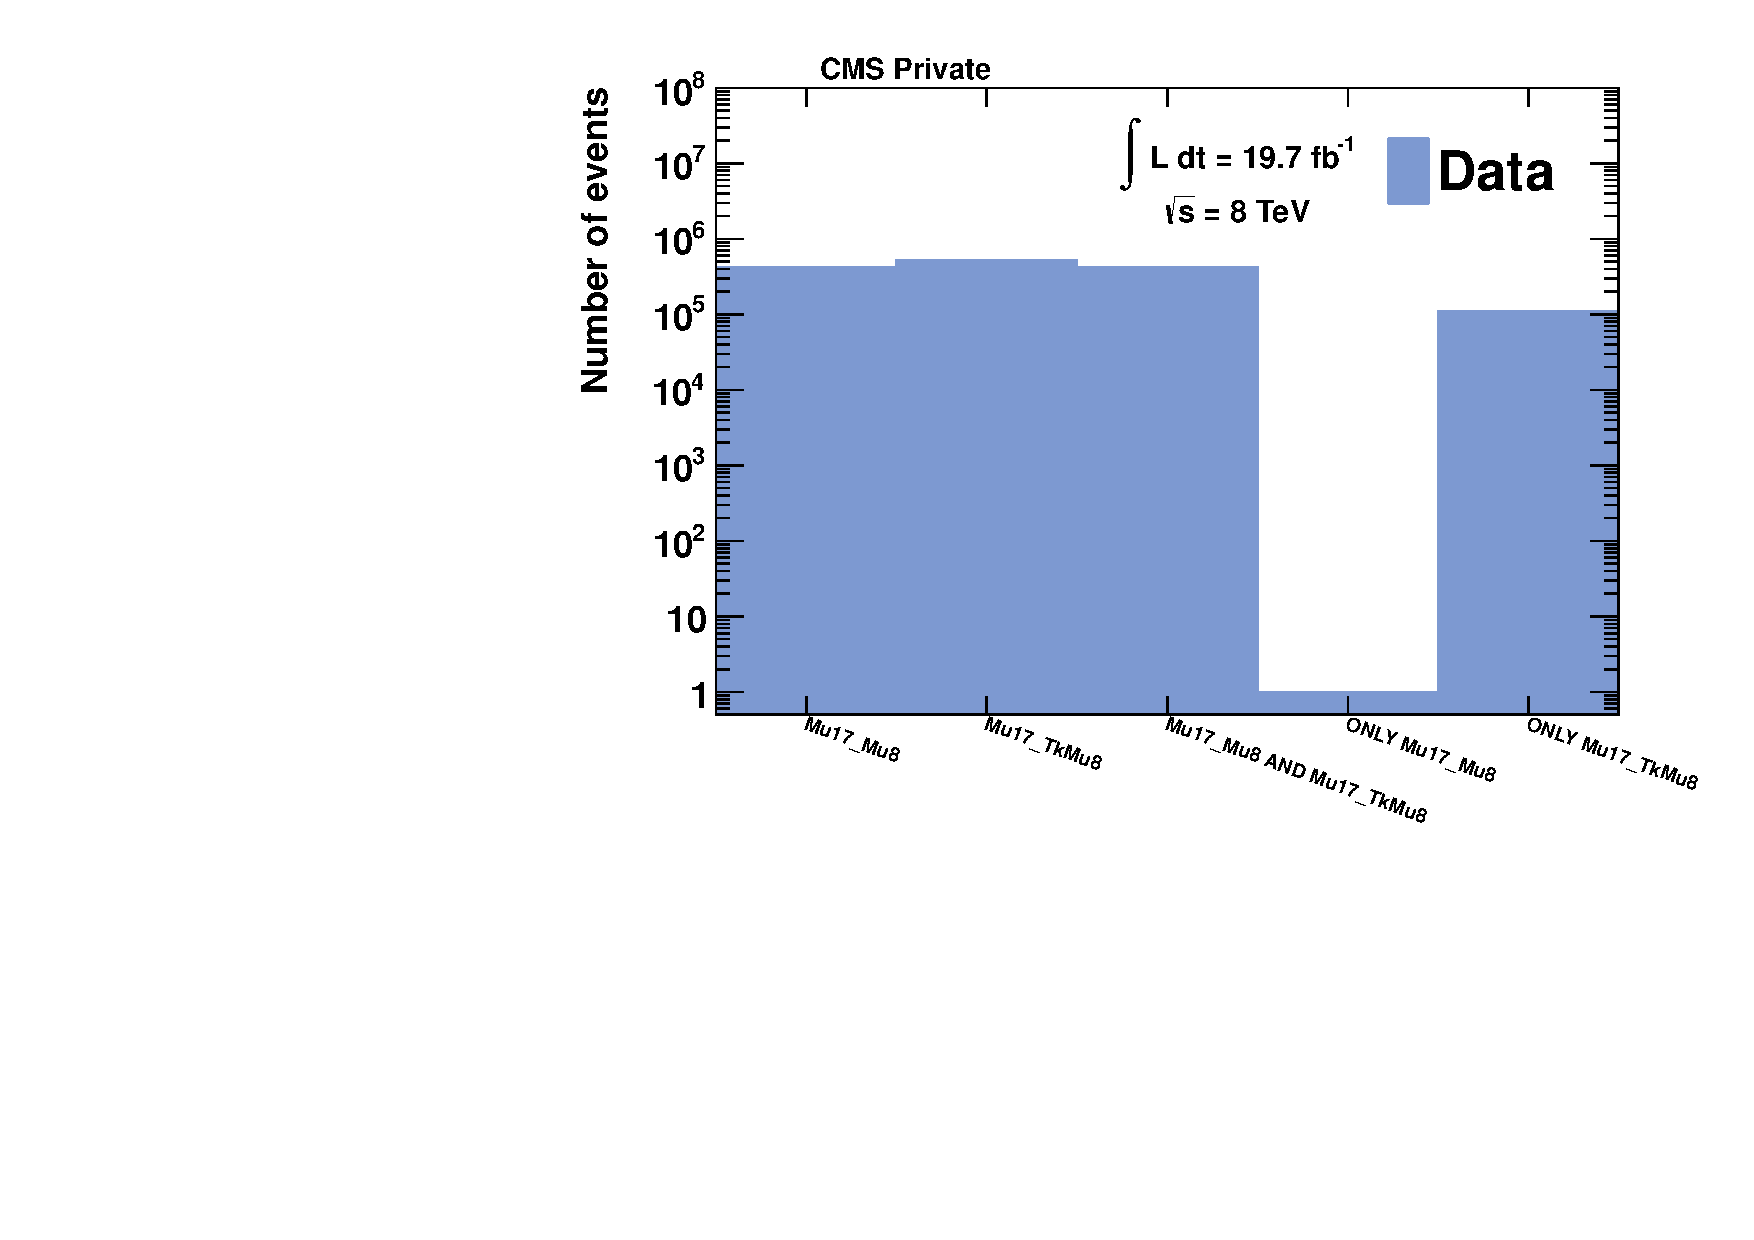
\includegraphics[width=0.8\textwidth]{plots/dycut_matched.pdf}
  \caption{Each bin represents the number of data events passing the various trigger combinations given on the $x$-axis. All four runs of 2012 (Tab.~\ref{tab:data}) are included in this distribution.}
  \label{fig:matched}
\end{figure}

\noindent The first two bins of the distribution show the results for each individual trigger. By raw numbers, \verb+HLT_Mu17_TkMu8+ is in the lead in terms of overall efficiency. To get en estimate of the overlap, the third bin shows the case when both triggers are required at once. With the number of events being quite similar to the one for \verb+HLT_Mu17_Mu8+, one can conclude that almost all events in the first bin are contained in the second one as well. To further quantify this conclusion, the fourth and fifth bin display the event count of \textit{only} one out of the two being triggered. Comparing the contents of these bins with the previous ones, the additional efficiency yielded by using \verb+HLT_Mu17_Mu8+ in addition to \verb+HLT_Mu17_TkMu8+ can be estimated. With it being only of the order of $\mathcal{O}(10^{-5})$, this analysis uses the latter trigger exclusively.


\section{Muon Identification}
\label{sec:muonid}

The recipe employed for muon identification has been developed by the Muon POG. The current recommendations can be found on the respective TWiki Website~\cite{muonpog}. Its main purpose is to differentiate between prompt and non-prompt muons.

Since the analysis expects a low amount of statistics in the final distributions, the tight muon ID~\cite{muonid1, muonid2} has been chosen. This is the most strict criterion given by the physics object group, thus being the best choice to prevent misidentification. The requirements are given below and apply to all muons within the intermediate energy range.

\begin{itemize}
\item \textbf{Global Muon} - The object is required to be identified as global muon. As discussed in the object reconstruction (Sec.~\ref{sec:objreco}), this means that a set of hits in the muon system has to be matched to a compatible set in the tracker. With mostly muons being able to pass through the inner detector layers, this serves as a major tool for identifying muons.
\item \textbf{Particle Flow Muon} - As outlined in the object reconstruction, particle flow algorithm considers the measurements from all sub-detectors. By combining the information of an entire event, the accuracy of particle identification is improved.
\item \textbf{Muon Track} $\mathbf{\chi^2 / N_{\textbf{dof}} < 10}$ - The fit of the trajectory has to describe the hits reasonably well. This is meant to protect against muons stemming from an decay in flight, as well as hadronic components passing the HCAL~\cite{muonidcosmic}. In both cases the trajectory is likely not to have a match in the tracker region.
\item $\mathbf{N_{\textbf{Muon Chambers}} > 0}$ - For the same purpose at least one muon chamber has to be part of the global fit. 
\item $\mathbf{N_{\textbf{Matched Stations}} > 1}$ - Requiring at least two muon stations to have a muon segment hit provides consistency with the trigger\footnote{A reasonable estimate for the transverse momentum requires a minimum of three hits. Without a well reconstructed transverse momentum, the trigger threshold becomes meaningless as it is based upon that.}. Once again, this aids against punch-through particles and also against general mismatches of tracks.
\item $\mathbf{d_{xy} < 2\,\textbf{mm}}$ - The impact parameter in the transverse plane, in respect to the primary vertex, has to be low. Both decays in flight and cosmic muons are unlikely to meet this criterion~\cite{muonidcosmic}.
\item $\mathbf{d_z < 5\,\textbf{mm}}$ - The longitudinal distance towards the primary vertex also has to be low for the same reasons.
\item $\mathbf{N_{\textbf{Pixel Hits}} > 0}$ - Since in flight decays may not have hits in the pixel detector, this requirement provides further suppression and association to a single vertex.
\item $\mathbf{N_{\textbf{Tracker Layers}} > 0}$ - A certain amount of tracker layers needs to be hit for a precise transverse momentum measurement. Additionally, the same logic as for the hits in the pixel detector applies.
\end{itemize}

The detector coverage only ensure a consistent momentum resolution for muons in the $\eta$-region up to 2.1 (C.f. cha.~\ref{cha:experiment}). Hence the analysis limits itself to this region. Together with a minimum transverse momentum set by the trigger, these are the basic criteria for object selection with regards to muons. They will be used and expanded upon in the event selection (Sec.~\ref{cha:eventsel}). 


\section{Jet \& Missing Transverse Energy Identification}
\label{sec:jetid}

For selecting jets and missing transverse energy, this analysis relies on the work of the JetMET POG~\cite{jmepog}. Jets are reconstructed using the anti-$k_{\text{T}}$ ($\Delta R < 0.5$) and particle flow algorithm. The latter is also responsible for the calculation of the missing transverse energy. The recommended loose working point~\cite{jetid, jetidpf} has been chosen with regards to jet requirements. The idea is to support the event selection which uses muons as its basis, while giving confidence for the final state selection. The values are given below.

\begin{itemize}
\item \textbf{Number Of Constitutients} $\mathbf{> 1}$ - Amount of particle components of the jet.
\item \textbf{Neutral Hadron Fraction} $\mathbf{< 0.99}$ - Fraction of the energy deposited in the HCAL by neutral particles.
\item \textbf{Charged Hadron Fraction} $\mathbf{> 0}$ - Fraction of the energy deposited in the HCAL by charged particles.
\item \textbf{Neutral EM Fraction} $\mathbf{< 0.99}$ - Fraction of the energy deposited in the ECAL by neutral particles.
\item \textbf{Charged EM Fraction} $\mathbf{< 0.99}$ - Fraction of the energy deposited in the ECAL by charged particles.
\item \textbf{Charged Multiplicity} $\mathbf{> 0}$ - Number of charged jet components.
\end{itemize}

For the transverse momentum threshold and spatial coverage $15\,\text{GeV}$ and $|\eta|  < 2.4$ are required. A spatial distance of at least $\Delta R > 0.05$ to a selected muon is being ensured as well. This is meant to prevent valid muons from being misreconstructed as particle flow jets. 

\section{Electron Identification}
\label{sec:eleid}

For selecting electrons, the Egamma POG recommendations are employed. These are taken from and can be found on yet another TWiki Website~\cite{egammaid}. Since electron identification is only used for vetoing against potentially misreconstructed events, they are of lower importance compared to the previously discussed physics objects. The chosen medium working point is similar to VBTF 80 working points and has the following requirements for the barrel (encaps) region. 


\begin{itemize}
\item $\mathbf{\Delta \eta_{\textbf{SC}} < 0.004 (0.007)}$ - $\eta$-distance to supercluster.
\item $\mathbf{\Delta \phi_{\textbf{SC}} < 0.06 (0.03)}$ - $\phi$-distance to supercluster.
\item $\mathbf{\sigma_{I\eta I\eta} < 0.01 (0.03)}$ - Size of the spread of the supercluster; measured in units of crystals.
\end{itemize}

A supercluster (\textbf{SC}) describes an $\eta$-region of ECAL entries triggered by an electron. Due to the trajectory being bent, the electron emits photons resulting in these additional hits in the adjacent ECAL cells.

\begin{itemize}
\item $\mathbf{H / E < 0.12 (0.10)}$ - Ratio of energy measurement in HCAL to ECAL.
\item $\mathbf{d_{0, \textbf{vtx}} < 0.02}$ - Transverse distance to primary vertex. 
\item $\mathbf{d_{z, \textbf{vtx}} < 0.1}$ - Longitudinal distance to primary vertex.
\item $\mathbf{1/E - 1/p < 0.05}$ - Difference of the inverse energy and momentum.
\item $\mathbf{\textbf{Combined I}_{\textbf{rel, PF}} < 0.15}$ - Combined relative isolation.
\item \textbf{Missing Hits} $\mathbf{<= 1}$ - Number of expected tracker hits that are missing.
\item \textbf{Vertex Fit Probability} $\mathbf{> 10^{-6}}$ - Likelihood of the electron being matched to a conversion vertex.
\end{itemize}

Isolation describes the amount of energy in close vicinity $\Delta R = 0.3$ to the particle's trajectory. Section~\ref{sec:muonqualy} will go into more detail on this topic. To match the electron trigger's settings, the individual tracker, ECAL and HCAL entries are also required to have an isolation less than 0.2, respectively.

%%% Local Variables: 
%%% mode: latex
%%% TeX-master: "document"
%%% End: 
